% BDE Guide --- Chapter 4: College Core
\chapter{College Core: The Professional Spine}
\label{ch:college-core}

\begin{quote}
\emph{``College Core is the bridge from classroom to workplace.''} These are not BDEs --- they are compulsory professional modules owned by CCDS. Confusing College Core with BDE is a common audit error; this chapter makes the distinction crisp.
\end{quote}

\noindent\fbox{\parbox{\dimexpr\linewidth-2\fboxsep-2\fboxrule}{%
\textbf{From zero: College Core defined.} College Core $=$ the \emph{common professional spine} for every CCDS BSc student (CS, AI, Data Science). It is \emph{not} optional, \emph{not} BDE, and \emph{not} MPE. We cover each component---purpose, AU, timing, and assessment---then contrast SC3099 vs.\ SC4079.}}
\vspace{0.4em}

\section*{Learning Outcomes}
After this chapter you will be able to:
\begin{enumerate}[label=(L\arabic*)]
    \item list the College Core components, AU, and typical semester for each;
    \item explain the purpose of SC1003, HW0288, SC3920, and the SC3099/SC4079 projects;
    \item distinguish SC3099 Capstone (Programme Core, Y3 S1) from SC4079 FYP (MPE, Y4);
    \item state prerequisites, grading, and workload expectations for each College Core course;
    \item avoid the common mistake of counting a College Core course as BDE.
\end{enumerate}

% ============================================================
\section{What Is College Core?}
\label{sec:what-college-core}

\begin{definition}[College Core (Professional Series)]
College Core is a CCDS-level requirement of 16~AU (curriculum-page bucketing; the alternative PDF Foundational-Core summary shows 15~AU for the same courses --- the 1~AU delta is a boundary shift with BDE, total 135~AU invariant). Every CCDS BSc student --- CS, AI, Data Science --- takes the same College Core spine. In the curriculum-page bucketing it comprises:
\begin{center}
\small
\renewcommand{\arraystretch}{1.25}
\begin{tabular}{@{}l c l p{5.5cm}@{}}
\toprule
Course & AU & When & Purpose \\
\midrule
SC1003 Intro to Computational Thinking \& Programming & 3 & Y1 S1 & Foundational programming \& problem solving \\
HW0288 Engineering Communication & 2 & Y3 & Professional writing, presentation, teamwork \\
SC3920 Professional Internship & 10 & Y3 S2 & Full-time industry attachment (graded) \\
\midrule
\multicolumn{4}{@{}l}{\footnotesize Plus 1~AU institutional rounding / bridging that appears as BDE in the PDF bucketing.} \\
\bottomrule
\end{tabular}
\end{center}
SC3099 (Capstone, 4~AU, Y3 S1) and SC4079 (FYP, 8~AU, Y4) are \emph{narratively} part of the professional spine but bucketed differently in the official summaries: SC3099 is Programme Core (Core 47~AU in the PDF) and SC4079 is MPE (see below). Table~\ref{tab:au-buckets} in the Appendix shows both bucketings side-by-side.
\end{definition}

\begin{figure}[h]
\centering
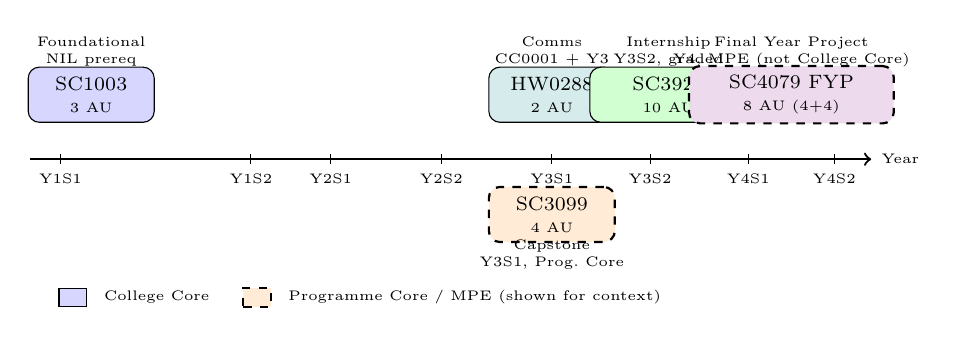
\begin{tikzpicture}[scale=0.78,every node/.style={font=\scriptsize}]
% Timeline of College Core
\draw[thick,->] (-0.5,0) -- (13.2,0) node[anchor=west,font=\tiny] {Year};
\foreach \x/\l in {0/Y1S1,3.1/Y1S2,4.4/Y2S1,6.2/Y2S2,8.0/Y3S1,9.6/Y3S2,11.2/Y4S1,12.6/Y4S2} \draw (\x,0.08)--(\x,-0.08) node[below,font=\tiny] {\l};
% SC1003
\node[draw,fill=blue!16,rounded corners=4pt,minimum width=1.6cm,minimum height=0.7cm,align=center] at (0.5,1.05) {SC1003\\{\tiny 3 AU}};
\node[font=\tiny,align=center] at (0.5,1.75) {Foundational\\{\tiny NIL prereq}};
% HW0288
\node[draw,fill=teal!16,rounded corners=4pt,minimum width=1.6cm,minimum height=0.7cm,align=center] at (8.0,1.05) {HW0288\\{\tiny 2 AU}};
\node[font=\tiny,align=center] at (8.0,1.75) {Comms\\{\tiny CC0001 + Y3}};
% SC3099 (dashed = Programme Core)
\node[draw,dashed,thick,fill=orange!16,rounded corners=4pt,minimum width=1.6cm,minimum height=0.7cm,align=center] at (8.0, -0.9) {SC3099\\{\tiny 4 AU}};
\node[font=\tiny,align=center] at (8.0,-1.55) {Capstone\\{\tiny Y3S1, Prog.\ Core}};
% SC3920
\node[draw,fill=green!18,rounded corners=4pt,minimum width=2.0cm,minimum height=0.7cm,align=center] at (9.9,1.05) {SC3920\\{\tiny 10 AU}};
\node[font=\tiny,align=center] at (9.9,1.75) {Internship\\{\tiny Y3S2, graded}};
% SC4079 (dashed = MPE)
\node[draw,dashed,thick,fill=violet!14,rounded corners=4pt,minimum width=2.6cm,minimum height=0.7cm,align=center] at (11.9,1.05) {SC4079 FYP\\{\tiny 8 AU (4+4)}};
\node[font=\tiny,align=center] at (11.9,1.75) {Final Year Project\\{\tiny Y4, MPE (not College Core)}};
% Legend
\node[draw,fill=blue!16,minimum width=0.35cm,minimum height=0.22cm] at (0.2,-2.25) {};
\node[font=\tiny,anchor=west] at (0.55,-2.25) {College Core};
\node[draw,dashed,thick,fill=orange!16,minimum width=0.35cm,minimum height=0.22cm] at (3.2,-2.25) {};
\node[font=\tiny,anchor=west] at (3.55,-2.25) {Programme Core / MPE (shown for context)};
\end{tikzpicture}
\caption{College Core timeline (solid) with SC3099/SC4079 shown dashed for context. Y3 S2 internship dominates that semester --- no BDE alongside it.}
\label{fig:college-core-timeline}
\end{figure}

\begin{remark}[Bucketing confusion]
If you compare the curriculum page (College Core 16~AU) with the PDF summary (Foundational Core 15~AU + Core 47~AU that includes SC3099), the 1~AU difference is the same BDE-boundary shift seen in Ch.~\ref{ch:bde-overview}. Degree Audit reconciles both views; the course list is identical.
\end{remark}

% ============================================================
\section{The Three College Core Courses in Detail}
\label{sec:college-courses}

\subsection{SC1003 Introduction to Computational Thinking \& Programming (3~AU)}
\paragraph{When \& prerequisites.} Y1 S1, no prerequisites (NIL). Co-requisite for SC1004 (Linear Algebra for Computing).

\paragraph{What it is.} Your first programming course: problem decomposition, algorithmic thinking, Python (or cohort language), basic data structures, testing, and debugging. It also co-introduces the mathematical maturity (sets, logic) that MH1812 and SC2001 will formalise.

\paragraph{Workload.} 3~h lecture + 1~h tutorial + 2~h lab per week is typical; continuous assessment (labs, quizzes, mini-project) plus a final exam. Pass SC1003 early --- it unlocks SC1007, SC1008, SC2002, and indirectly most of Y2.

\paragraph{Why it is College Core, not BDE.} It is foundational for every CCDS programme; without it, downstream cores have no programming base. Counting it as BDE would undercount your core AU.

\subsection{HW0288 Engineering Communication (2~AU)}
\paragraph{When \& prerequisites.} Y3, prerequisites CC0001 (Inquiry \& Communication) \emph{and} Year~3 standing. Offered by the School of Humanities (HSS) for CCDS.

\paragraph{What it is.} Professional communication: technical writing (reports, proposals), oral presentation, visual communication, and teamwork dynamics. Assessment is heavily continuous --- presentations, group report, peer review --- with little or no final exam.

\paragraph{Why it matters for CS.} Code is read more than written; so are design docs, incident reports, and product specs. HW0288 is the only compulsory course that grades your ability to explain technical work to mixed audiences. Recruiters who ask for ``strong communication skills'' are asking for what this course practises.

\paragraph{Not a BDE.} HW0288 is compulsory College Core; you cannot S/U it as a BDE or replace it with another HSS course.

\subsection{SC3920 Professional Internship (10~AU, Graded)}
\paragraph{When \& prerequisites.} Y3 S2, Year~3 standing. Full-time, typically 20--24 weeks.

\paragraph{What it is.} A graded, credit-bearing attachment in industry (or approved research/overseas internship). You are assessed on work performance (employer evaluation), a written report, and often a presentation. The grade counts toward GPA and honours classification.

\paragraph{Key rules.}
\begin{itemize}
    \item \textbf{Graded, not Pass/Fail.} Unlike some universities' internships, SC3920 carries a letter grade that affects GPA. Treat it as a 10~AU course, not a ``break''.
    \item \textbf{Full-time commitment.} Do not plan BDEs or heavy MPEs alongside SC3920. The official guidance is to take at most one additional small course (often an ICC or online module) if your employer schedule permits; many students take none.
    \item \textbf{Timing alternatives.} A small number of students intern in Y3 S1 or Y4 by arrangement; this shifts SC3099/MPE timing. Confirm with CCDS Undergraduate Office before moving it.
    \item \textbf{Overseas / research internships} are possible but require prior approval and may have different deliverables.
\end{itemize}

\begin{center}
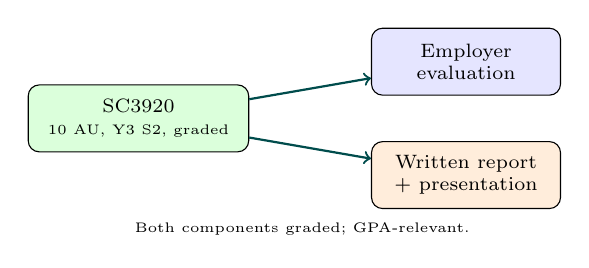
\begin{tikzpicture}[scale=0.80,every node/.style={font=\scriptsize}]
\node[draw,fill=green!14,rounded corners=4pt,minimum width=2.8cm,minimum height=0.85cm,align=center] (a) at (0,0) {SC3920\\{\tiny 10 AU, Y3 S2, graded}};
\node[draw,fill=blue!10,rounded corners=4pt,minimum width=2.4cm,minimum height=0.85cm,align=center] (b) at (5.2,0.9) {Employer\\evaluation};
\node[draw,fill=orange!14,rounded corners=4pt,minimum width=2.4cm,minimum height=0.85cm,align=center] (c) at (5.2,-0.9) {Written report\\+ presentation};
\draw[->,thick,teal!60!black] (a) -- (b);
\draw[->,thick,teal!60!black] (a) -- (c);
\node[font=\tiny,align=center,fill=white,inner sep=2pt] at (2.6,-1.75) {Both components graded; GPA-relevant.};
\end{tikzpicture}
\end{center}

% ============================================================
\section{SC3099 vs.\ SC4079: Two Different Projects}
\label{sec:capstone-vs-fyp}

This is the most confused pair in the programme. They are different courses, different years, different buckets, and different honours implications.

\begin{table}[h]
\centering
\small
\renewcommand{\arraystretch}{1.25}
\begin{tabular}{@{}p{3.2cm} p{4.7cm} p{4.7cm}@{}}
\toprule
 & \textbf{SC3099 Capstone Project} & \textbf{SC4079 Final Year Project (FYP)} \\
\midrule
AU & 4~AU & 8~AU (4 + 4 across Y4 S1 \& S2) \\
Bucket & Programme Core (Core 47) & MPE (counts toward 35~AU MPE) \\
When & Y3 S1, Year~3 standing & Y4 S1--S2, Year~4 standing \\
Team & Team-based (3--5 students) & Individual (supervised by faculty) \\
Deliverable & Integrated system / product + report + demo & Research or engineering thesis + defence \\
Grading & Team + individual components & Individual; supervisor + examiner \\
Honours & Required for all & Required for Highest Distinction; alternative is 3 extra MPE (see below) \\
\bottomrule
\end{tabular}
\caption{SC3099 vs.\ SC4079 at a glance. Do not confuse them; Degree Audit lists them separately.}
\label{tab:capstone-vs-fyp}
\end{table}

\begin{remark}[FYP-or-3-MPE rule (PDF Notes 2--3)]
To satisfy the 35~AU MPE requirement you have two paths:
\begin{itemize}
    \item \textbf{FYP path (standard):} 27~AU of MPE courses (9 courses $\times$ 3~AU, with $\ge$4 at 4000-level) + SC4079 (8~AU) $=$ 35~AU MPE. Required for Highest Distinction eligibility.
    \item \textbf{Non-FYP path:} 27~AU of MPE courses + 3 \emph{additional} MPE courses (9~AU) $=$ 36~AU MPE. Total degree becomes 136~AU unless BDE is adjusted per Degree Audit; confirm with your advisor. Highest Distinction is not attainable on this path.
\end{itemize}
Either way, SC3099 is \emph{always} required as Programme Core --- it is not interchangeable with SC4079.
\end{remark}

\begin{figure}[h]
\centering
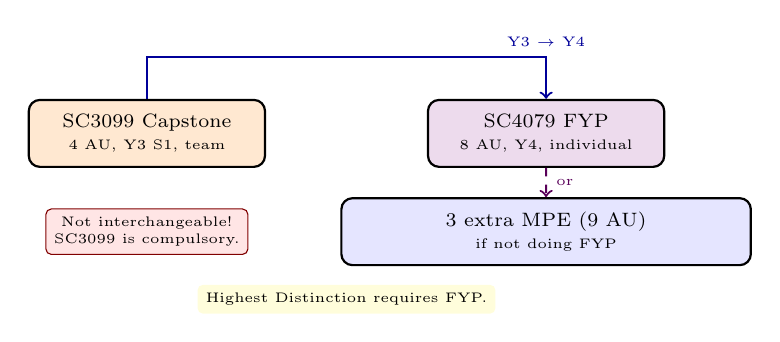
\begin{tikzpicture}[scale=0.78,every node/.style={font=\scriptsize},
  box/.style={draw,thick,rounded corners=4pt,align=center,minimum height=0.85cm,inner sep=4pt}]
\node[box,fill=orange!18,minimum width=3.0cm] (c) at (0,0) {SC3099 Capstone\\{\tiny 4 AU, Y3 S1, team}};
\node[box,fill=violet!14,minimum width=3.0cm] (f) at (6.5,0) {SC4079 FYP\\{\tiny 8 AU, Y4, individual}};
\node[box,fill=blue!10,minimum width=5.2cm] (alt) at (6.5,-1.6) {3 extra MPE (9 AU)\\{\tiny if not doing FYP}};
\draw[->,thick,blue!60!black] (c) -- ++(0,1.25) -| (f) node[midway,above,font=\tiny] {Y3 $\to$ Y4};
\draw[->,thick,dashed,violet!70!black] (f) -- (alt) node[midway,right,font=\tiny] {or};
\node[font=\tiny,align=center,fill=red!10,rounded corners=2pt,inner sep=3pt,draw=red!50!black] at (0,-1.6) {Not interchangeable!\\SC3099 is compulsory.};
\node[font=\tiny,align=center,fill=yellow!14,rounded corners=2pt,inner sep=3pt] at (3.25,-2.7) {Highest Distinction requires FYP.};
\end{tikzpicture}
\caption{SC3099 and SC4079 are sequential, not alternative. The \emph{alternative} is FYP vs.\ 3 extra MPE for the MPE bucket.}
\label{fig:capstone-fyp-flow}
\end{figure}

% ============================================================
\section{Chapter Notes}
Course details per CCDS BSc (Hons) in Computer Science study plan (AY2024--25), NTU Course Catalogue entries for SC1003/HW0288/SC3920/SC3099/SC4079, and PDF Notes 1--3 on MPE/FYP. Assessment mixes vary by semester; confirm in the course outline. Internship duration and grading per CCDS Undergraduate Office guidelines at time of writing.

% ============================================================
\section{Exercises}
\label{sec:ch04-exercises}
\begin{enumerate}[label=E4.\arabic*, leftmargin=*, itemsep=0.8em]
    \item \textbf{Bucket check.} A student lists SC1003 as a BDE in their plan. Why is this wrong, and which bucket does it belong to?
    \item \textbf{Capstone vs.\ FYP.} State two differences between SC3099 and SC4079 (AU, bucket, timing, or team structure).
    \item \textbf{Internship planning.} Can you take a 3~AU BDE alongside SC3920 in Y3 S2? What is the recommended load that semester?
    \item \textbf{Honours rule.} You want to graduate with Highest Distinction but prefer not to do an FYP. Is this possible? What does the programme require?
\end{enumerate}
% End of Chapter 4
